\chapter{Analysis}
\label{analysis}
Used data structures and algorithms in the implemented compiler are discussed in this chapter.
\section{Format of relational algebra}

In this section we present relation algebra operators which are the input of the compiler. Our relational algebra contains the following operators:
\begin{enumerate}
\item Projection -- we used extended projection $\pi_L$ which removes columns, computes new ones using expressions and renames attributes.

\item Table reading operator which is a leaf of the algebra tree. For this operator we need to provide the following arguments:
\begin{itemize}
\item table name.
\item information about indices (name, columns and sort order).
\item read columns.
\end{itemize}
\item Join - we used theta join $\Join_C$ operator where $C$ is condition having following format:
\begin{itemize}
\item Condition can be empty and in this case join represents Cartesian product.
\item $a_1=b_1~and~a_2=b_2~and~a_3=b_3~and...and~a_n=b_n$, where $a_k$ belongs to the first relation and $b_k$ belongs to the other relation.
\item $a_1\oplus b \ominus a_2$, where $a_1$ and $a_2$ belongs to one input and $b$ belongs to second input. Signs $\oplus$ and $\ominus$ mean $<$ or $\leq$.

\end{itemize}

In addition to condition, we need to specify output attributes of the join. These attributes can come from both inputs and we can optionally assign them a new name. Assigning new attribute name is useful when some of the attributes have the same name.

The other types of joins are not directly supported, but they can be replaced with the cross join followed by selection.
\item Anti join operator which was not presented with other algebra join operators. Output of the expression $R \ltimes_C S$ is relation with tuples from $R$, for which do not exist any tuple from $S$ that satisfies condition $C$. We can use join and anti join to express outer join.
 
The anti join can replace difference operator. The expression $R-S$ equals $R \ltimes_C S$, where $C$ is condition that equates each pair of attributes of $R$ and $S$ with the same name.
 
Including the anti join in our relation algebra eliminates the need of usage the outer join and the difference and our relational algebra is simpler.

Condition $C$ of anti join $R \ltimes_C S$ has the following format:
\begin{itemize}
\item $a_1=b_1~and~a_2=b_2~and~a_3=b_3~and...and~a_n=b_n$, where $a_k$ belongs to first the relation and $b_k$ belongs to the other relation.
\end{itemize}
In every anti join we need to specify its output attributes with optional new name. The anti join can output only columns from the first relation. 
\item Group operator $\gamma_L$, where L is non empty list of group attributes and aggregate functions. Supported aggregate functions are $min$, $max$, $sum$ and $count$. The function $avg$ is not supported but it can easily computed using $sum$ and $count$. All mentioned functions except $count$ take one input attribute and the function $count$ has empty input. 

As mentioned before, group operator is more general version of the duplicate elimination which is not included in our algebra.
\item Sort operator $\tau_L$, where $L$ is a non empty list of attributes with sort directions.
\item Bag union $\cup$. Both input relations has to have the same names and types of attributes. The set union can be computed using bag union and grouping operator for duplicates elimination.
\item Selection used in our algebra does not differ from selection from classical relational algebra.

\end{enumerate}

Designed relational algebra works with bags.

\section{Physical algorithms}

In this section we enumerate and describe compiler's output algorithms. We assume that execution environment has enough memory and physical operators do not have to store intermediate result on hard drive.

The following algorithms are generated by the compiler:
\begin{itemize}
\item \texttt{Filter} - this algorithm reads input tuples and outputs tuples satisfying given condition. Output does not have to be sorted the same way as input.
\item \texttt{Filter~keeping~order} - this algorithm reads input tuples and outputs tuples satisfying given condition. Output has to be sorted the same way as input.
\item \texttt{Hash~group} - operator groups tuples using hash table and for every group of tuples aggregate functions are computed.
\item \texttt{Sorted~group} - operator groups sorted tuples and computes aggregate functions. The input has to be sorted by group attributes.
\item \texttt{Column~operations} - this is an implementation of extended projection algebra operator. 
\item \texttt{Cross~join} - operator computes Cartesian product of two relations.
\item \texttt{Hash~join} - operator uses hash table to compute join of two relations $R$ and $S$ with condition $C$, where $C$ has the following format: $r_1=s_1~and~r_2=s_2~and~...~r_n=s_n$. Attributes $(r_1,r_2,...,r_n)$ belong to the relation $R$ and $(s_1,s_2,...,s_n)$ are from the relation $S$.
\item \texttt{Merge~equijoin} - algorithm takes advantage of sorted inputs to compute join with condition $C$, where $C$ has the same format like condition in \texttt{Hash~join}. 
\item \texttt{Merge~non~equijoin} - operator computes theta join with condition $a_1\oplus b \ominus a_2$, where $a_1$ and $a_2$ belong the first input and $b$ belongs to the second input. Signs $\oplus$ and $\ominus$ means $<$ or $\leq$. Input relations has to be sorted by the attributes in the join condition.
\item \texttt{Hash~anti~join} -  algorithm computes anti join with condition $C$  using hash table. Condition $C$ have the same format like condition in \texttt{Hash~join}
\item \texttt{Merge~anti~join} - operator takes advantage of sorted inputs to compute anti join with condition $C$, where $C$ has same format like condition in \texttt{Hash~join}. 
\item \texttt{Table~scan} - operator scans whole table from hard drive.
\item \texttt{Scan~and~sort~by~index} - operator scans whole table from hard drive using index. Output will be sorted by columns on used index.
\item \texttt{Index~Scan} - this algorithm uses index to read tuples from table satisfying given condition.
\item \texttt{Sort} - this algorithm sorts input. Input can be presorted and in this case, operator does only partial sorting.
\item \texttt{Union} - an implementation of bag union.

\end{itemize}


\section{Architecture}
The architecture of implemented tool is displayed in the figure~\ref{fig:compilerarchitecture}.

\begin{figure}[h!]
  \centering
    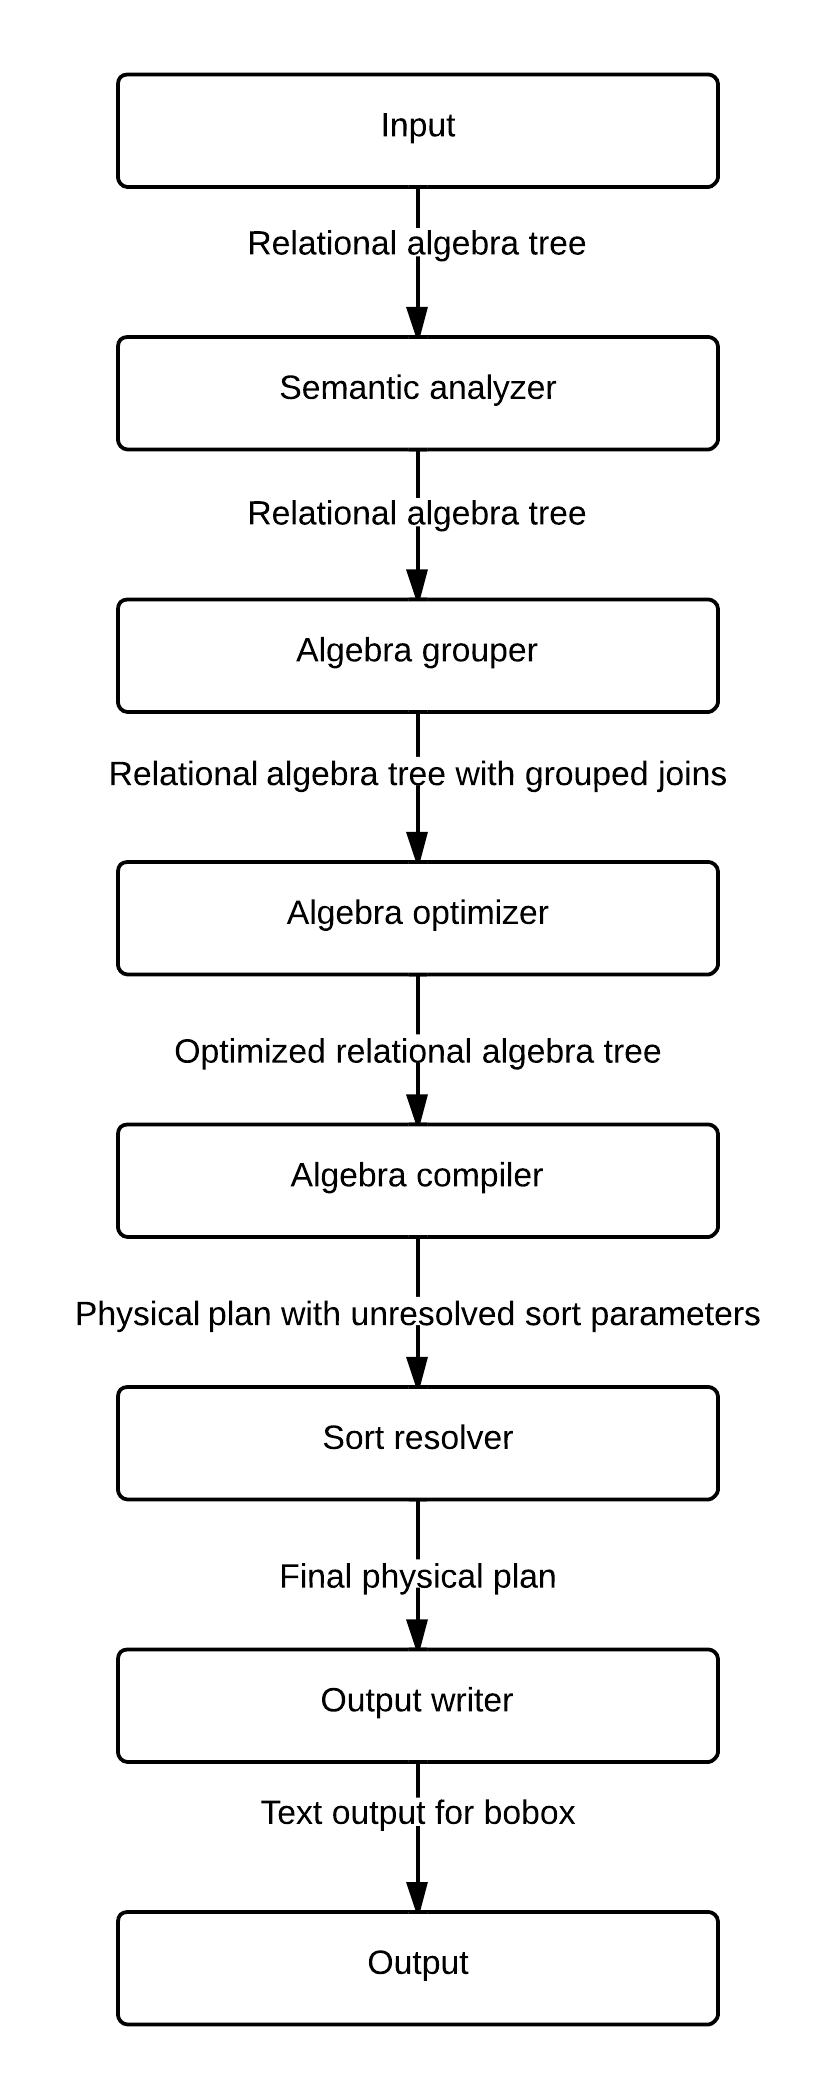
\includegraphics[width=0.5\textwidth]{compilerarchitecture}

      \caption{Compiler architecture.}
          \label{fig:compilerarchitecture}
\end{figure}

The relational algebra tree is read from XML file. For this format we decided for the following reasons:
\begin{itemize}
\item XML has tree--like structure.
\item For validation we only need to write schema.
\item There are already implemented tools for parsing.
\item There is no need to write input parser.
\end{itemize}

The relational algebra tree is checked in the \texttt{Semantic analyzer}. This component checks if all of the used attributes are in the input relation. \texttt{Semantic analyzer} searches for duplicate named attributes and reports them as an error. 

Semantically correct tree is processed by component \texttt{Algebra grouper} that groups neighboring joins into one. Thanks to this operation we can later choose the fastest way to join multiple relations.

Algebra tree with grouped joins is optimized. \texttt{Algebra optimizer} pushes the selections down the tree. This component also applies following operation:
\begin{itemize}
\item  $\sigma_C(R\Join_D S)= R\Join_{D~and~C} S$, where $C$ has the following format: $r=s$, $r$ belong to $R$ and $s$ belongs to $S$.
\end{itemize}

Optimized algebra tree is processed by \texttt{Algebra compiler}, which generates physical plan. This physical plan is not yet final. Its sort operator's parameters can represent multiple ways of sorting relation. When sorting relation before grouping, we have multiple possibilities how to sort current relation and we can decide later which way is the best.

Final plan is an output of the component named \texttt{Sort resolver}. This component resolved unknown sort order in sort operators and produces final plan, which is converted to Bobolang language.

Implemented tool  will be the back end of the compiler and it does not check column. We assume that the front end parsing the text will handle types. Types of columns are only copied to the output and we assume that column types do not contain any errors.

\section{Data structures}

Data structures used in implemented tool are presented in this section.

Relational algebra is stored in the polymorphic tree. Every node stores its parameters, pointer on the parent in the tree and pointers on its children node. No other structure was considered for this representation since this is efficient way to store logical plan. It allows to easily add and remove relational algebra operators.
The example of this representation can be found in the Figure~\ref{fig:groupalgebra}. It is representing simple query reading whole table. Read relation is grouped and aggregation functions are computed. The result is sorted at the end. Leaf of the tree stores the following information:
\begin{itemize}
\item List of indices on this table.
\item List of columns with their names, types and number of unique values
\item Size of the relation.
\end{itemize}
\begin{figure}[h!]
  \centering
    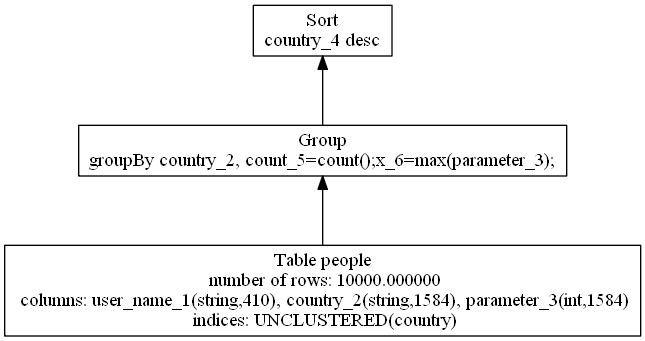
\includegraphics[width=0.8\textwidth]{groupalgebra}

      \caption{Example of relational algebra structure.}
          \label{fig:groupalgebra}
\end{figure}

We chose the same structure for physical plan. The advantage of storing physical plan into polymorphic tree is to ability to easily add new root node. The example of this representation can be found in the Figure~\ref{fig:groupplan}. This Figure contains one of the possible physical plans for relational algebra shown in the Figure~\ref{fig:groupalgebra}. For reading table we used algorithm \texttt{Table scan}, then we hashed input by requested columns. Result is sorted in \texttt{Sort} operator. Every nodes stores additional informations like output attributes, estimated run time and size of output relation.

\begin{figure}[h!]
  \centering
    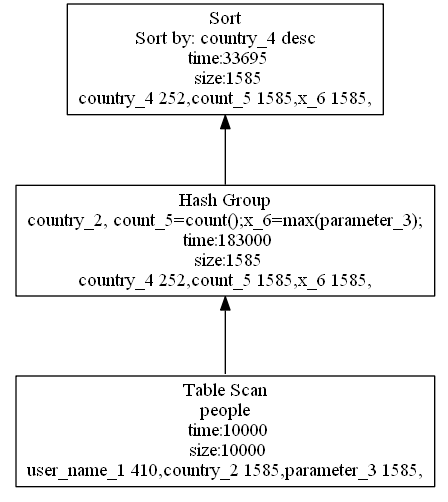
\includegraphics[width=0.6\textwidth]{groupplan}

      \caption{Example of physical plans structure.}
          \label{fig:groupplan}
\end{figure}

Physical and logical plans also contain expressions. The expressions are stored in polymorphic expression tree. Example of this structure can be found in the~Figure~\ref*{fig:expressiontree}.
\begin{figure}[h!]
  \centering
    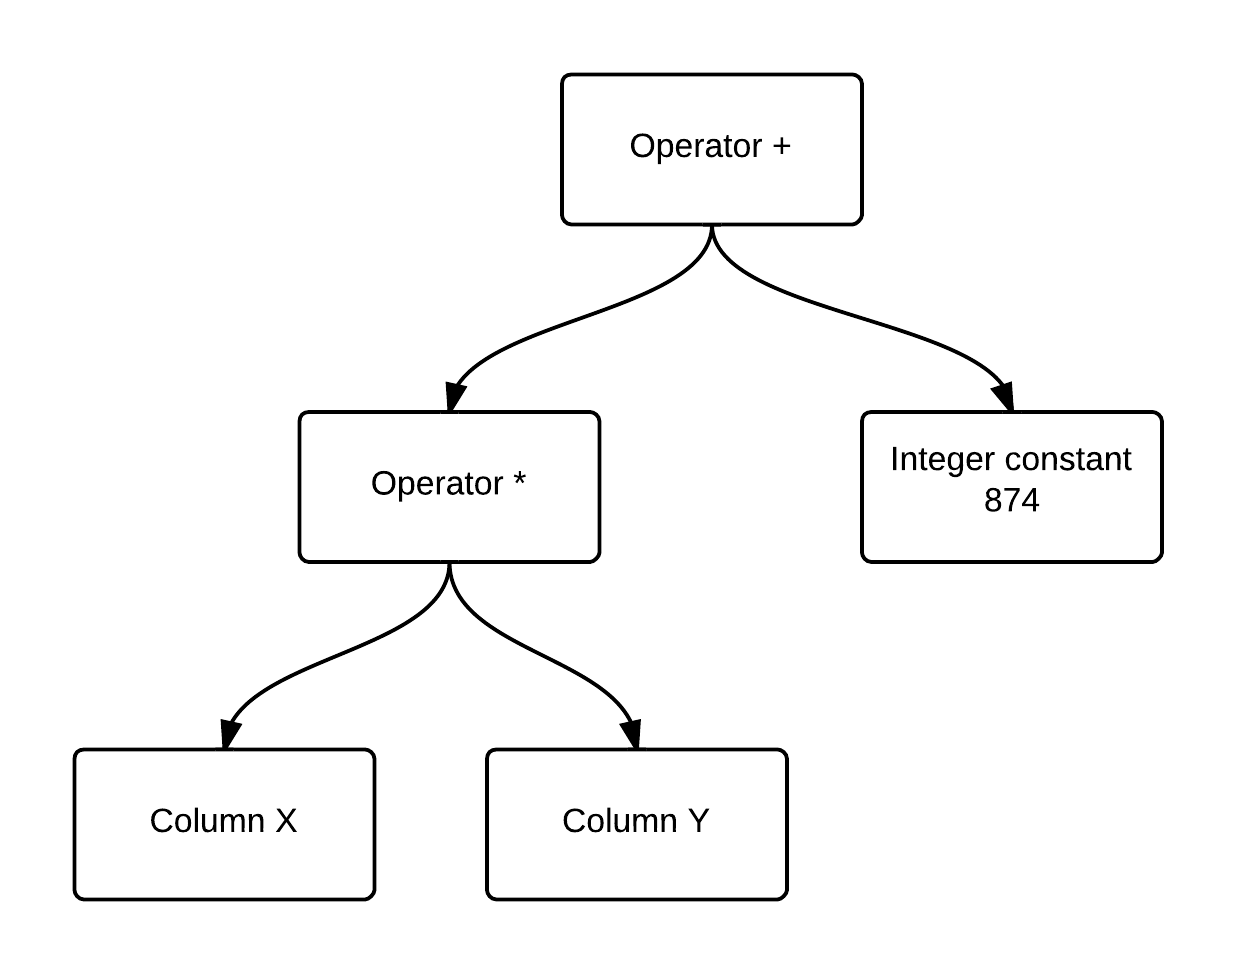
\includegraphics[width=0.6\textwidth]{expressiontree}

      \caption{Example expression tree representing expression  $X*Y+874$.}
          \label{fig:expressiontree}
\end{figure}

More complicated structure was used for storing sort parameters. This structure is stored in every physical sort operator to determine how the relation can be sorted. 

If we want to use sort based group operator and it groups by two columns, we have multiple possibilities for sorting relation. To use sort based algorithm for evaluating expression $\gamma_{x,y}(R)$ we can sort relation in four possible ways:
\begin{itemize}
\item $x:A,y:A$
\item $x:A,y:D$
\item $x:D,y:A$
\item $x:D,y:D$
\end{itemize}
$A$ means ascending and $D$ is abbreviation for descending.

There are multiple possibilities of sorting relation $R$ before applying  $R\Join_{r_1=s_1~and~r_2=s_2} S$. Relation $R$ can be sorted the following ways:
\begin{itemize}
\item $r_1,r_2$
\item $r_2,r_1$
\end{itemize}
Order, how to sort columns is arbitrary.

We also want to store information about equality of sort column. After applying merge join $R\Join_{r_1=s_1} S$, the result can sorted by $r_1$ or $s_1$. All this requirements were use to design structure for store sort parameters without enumerating all possible sort orders.

\begin{figure}[h!]
  \centering
    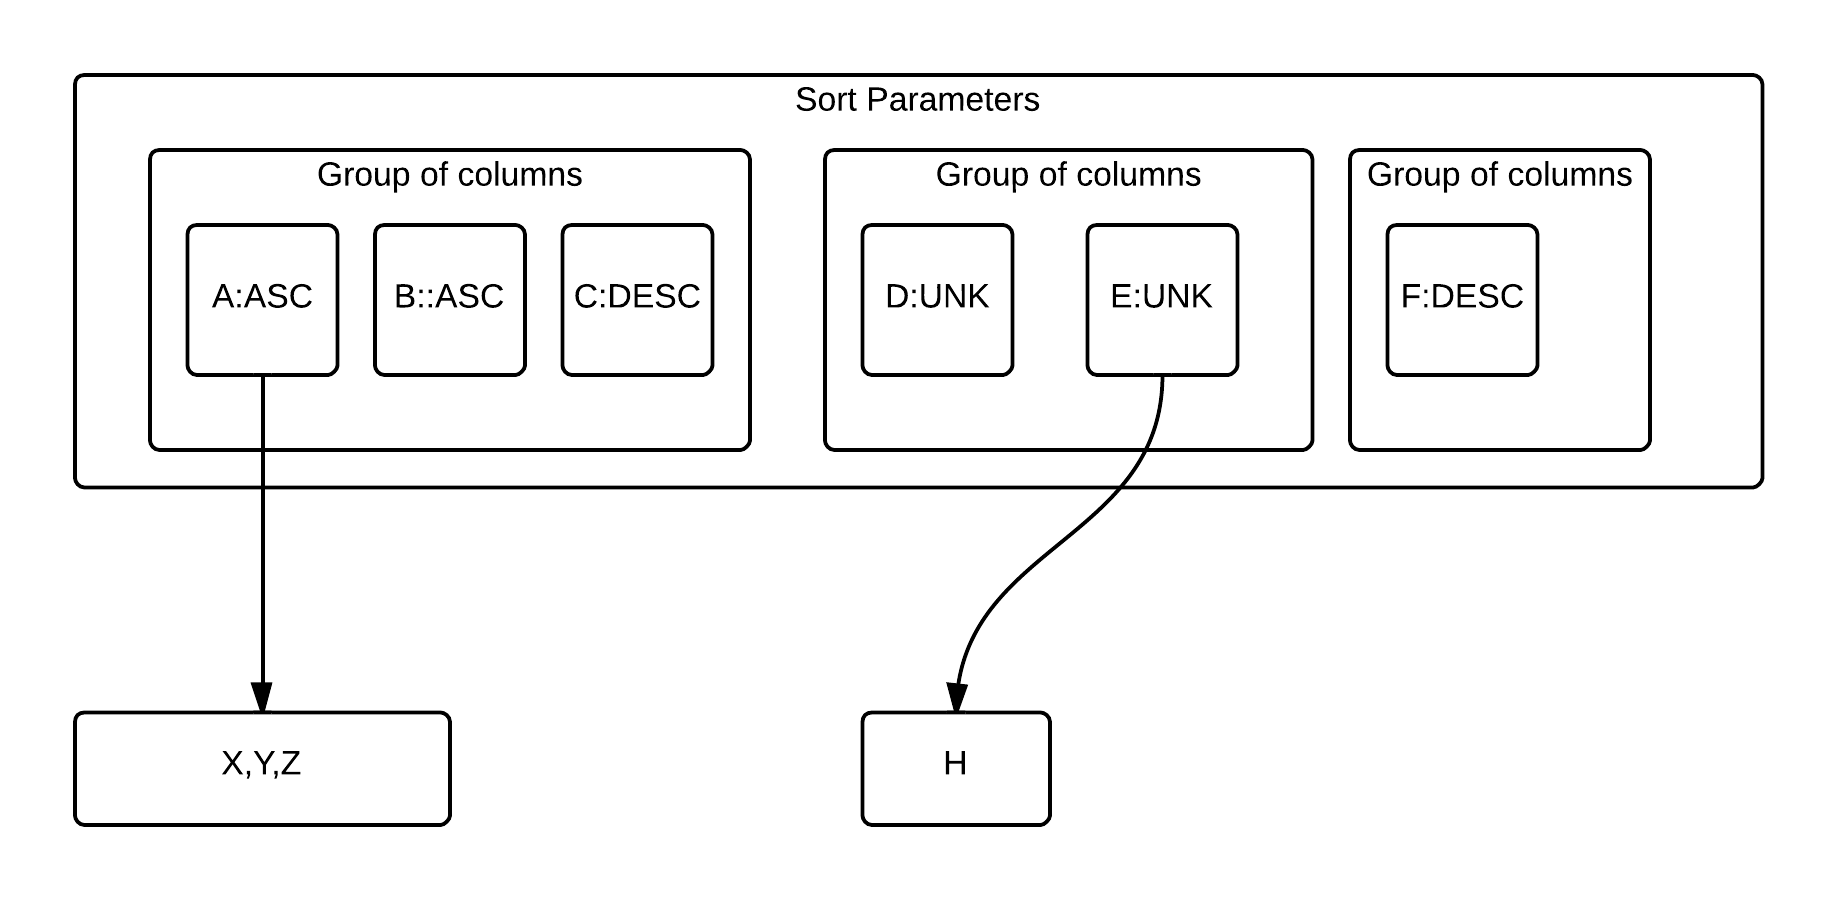
\includegraphics[width=0.9\textwidth]{sortparameters}

      \caption{Structure storing parameters for sort.}
          \label{fig:sortparameters}
\end{figure}

In figure \ref{fig:sortparameters} we display an example of sort parameters, which sorts by 6 columns. It contains one or more columns group. The order of columns groups cannot be changed. Order of columns in groups is arbitrary. It means that $F$ has to be on sixth place, but column $E$ can be on forth of fifth place. Every column contain information about sort order: $ASC$ (ascending), $Desc$ (descending) or $UNK$ (unknown - can be ascending or descending). We store list of equal attributes for every column. In case a projection operator removes columns $A$ from relation we can replace removed with attributes $X$, $Y$ or $Z$ in sort parameters.
The Figure~\ref{fig:sortparameters} represents many sort order possibilities, we enumerate only some of them:
\begin{enumerate}
\item $A:ASC,C:DESC,B:ASC,H:DESC,D:ASC,F:DESC$
\item $C:DESC,B:ASC,Z:ASC,H:DESC,D:DESC,F:DESC$
\item $B:ASC,C:DESC,A:ASC,E:ASC,D:DESC,F:DESC$
\item $C:DESC,B:ASC,Y:ASC,D:ASC,H:ASC,F:DESC$
\end{enumerate}



\section{Optimization}

In this section we describe algebra optimization, which was implemented to improve logical plan.

Before we start with optimizations we need to prepare logical plan. We group joins algebra nodes and expressions connected with $and$ and $or$. We work down the algebra tree. If we find join we convert to it grouped join. If one of its children is join, then we merge it with grouped join. This representation is used for choosing faster order join. Conditions are grouped the same way. From expression tree $a=2~and~(b=2~and~c=2)$ we create $AND(a=2,b=2,c=2)$. This representation is useful for splitting condition into simpler conditions.

We implemented very important optimization: pushing selection down the tree. Every selection is spitted into selections with simpler conditions. Every selection is moved down the tree as much as possible. In this phase we used the following rules ($\sigma_C$ is being pushed down):
\begin{enumerate}
\item $\sigma_C(\sigma_D(R))=\sigma_D(\sigma_C(R))$
\item $\sigma_C(\pi_L(R))=\pi_L(\sigma_C(R))$, it works only if $C$ does not contain new computed columns in extended projection. We also need to rename columns in condition $C$ in case projection renamed some of the condition columns.
\item  $\sigma_C(R \Join_D S)$ can be rewritten as
\begin{enumerate}
\item $\sigma_C(R) \Join_D S$ if $C$ contains only columns from $R$.
\item $R \Join_D \sigma_C(S)$ if $C$ contains only columns from $R$.
\item $R \Join_{D~and~C} S$ if $C$ is in form $a=b$ where $a$ belong the relation $R$ and $b$ comes from the relation $S$.
\end{enumerate}
\item $\sigma_C(R \ltimes_C S)=\sigma_C(R)\ltimes_C S$
\item $\sigma_C(R\cup S)=\sigma_C(R)\cup \sigma_C(S)$
\end{enumerate}

\section{Generating physical plan}

We try to choose easiest method for generating plans. The decision was between heuristic method and dynamic programming. It would be probably the same amount of source code. We chose dynamic programming, because it can give better results. Using this method, we generate all possible plans for each node and choose the fastest plan.

We process logical plan from leafs. For every leaf we generate all possible physical algorithms and we insert resulting plans into heap, where we keep $c$ fastest plans for current node. Variable $c$ is a constant set in compiler.
For every algebra node we used plans generated in its children to generate new plan. This way we continue up the algebra tree to the root.

Physical plans are compared based on estimated run time. Every operator stores its estimated run time. The sum of run times of all the operators is estimated run time of the whole physical plan.
Very important are equations, which compute estimated time for physical algorithm. They depend on size of input relation. Modifying them can resolve in getting better physical plans. For example, if physical algorithm \texttt{Hash join} takes too much time because it accesses random parts of memory, we can modify estimated times so sort with merge join will be preferred.

Crucial are informations about size of tables. If they are not provided in the input we use default value and physical plan will be probably worse. Other important parameter is number of unique values attribute. Size of join depends on it and since joins usually takes significant amount of time, it is important to have as precise values as possible. 

\subsection{Join order selecting algorithm}


In section \ref{joinOrder} we presented algorithm choosing join order. We should choose order of joins and then assign join algorithms. These operations are done in one phase for the following reason: In case we do not have information about table sizes, we cannot determine join order because all orders have the same estimated run time. In this situation we can start by joining relations which are sorted to get a faster plan.

We are using two algorithms dynamic programming and greedy algorithm. Version of used dynamic programming algorithm is enumerating all possible trees. This algorithm can output us very good plans but has exponential complexity. We use it only if number of joined relations in grouped join node is small. For joining more relations we use faster greedy algorithm which generated only left or right deep trees. Time complexity of greedy algorithm is not exponential but only polynomial.

Input in both algorithm is set of plans for every input join relation.

\subsubsection{Dynamic programing for selection join order}

We use a variation of algorithm described in section \ref{dymanicalgorithm}. Input relations are numbered from $1$ to $n$. We used table for storing plans, which key is non empty subset of the set ${1..n}$.

We only store $k$ best plans in every table cell, where $k$ is constant set in the compiler. It represents best plans that were created by joining inputs stored in the key of table entry.

We begin by storing input plans into table entry identified by the set containing number of input relation. In first iteration we fill tables entries, which key has two values, by combining plans from entries with key size $1$.

We continue by computing plans for entries, with key size $3,4...n$. Key of the current entry is spited in all possible pairs of non empty disjunctive subsets. We take plans from table entries identified with subsets and we generate new plans combining them. We only store $k$ fastest plans in the current table cell.
We continue until we compute plans for table entry identified by key ${1..n}$ These plans are our result.

Time complexity is at least exponential since we generate all subsets of $n$ relations, this value is $2^n$.


\subsubsection{Greedy algorithm for selection join order}
 This is a variation of algorithm described in section \ref{greedyalgorithm}. We begin by creating joins for every pair of relations. From created pairs we choose the fastest $k$ trees.
 
 In every iteration we generate new trees by adding new relation to every tree. Only $k$ best trees are chosen to continue to the following iteration. We iterate until we create join tree containing every input relation.
 
 Time complexity is $O(n^2)$. In every iteration we generate from every tree maximal $n$ new trees, but we keep only $k$ of them for next iteration. Number of iterations is $n-1$, because all trees grow by one in every iteration. Number $k$ is a constant so it does not change time complexity.
 
\subsection{Resolving sort parameters}

After we generated physical plan we need to decide what sort parameters in sort operator to use. We work down the tree and store information about sort order of the relation. Based on that, we adjust sort parameters or just choose the arbitrary sort order if possible.

